\documentclass[pra,12pt]{revtex4-2}
\usepackage{amsmath}
\usepackage{amssymb}
\usepackage{graphicx}
\usepackage{color}
\usepackage{mathrsfs}
\usepackage{enumerate}
\usepackage{epigraph}
\usepackage{framed}
\usepackage[pdfborder={0 0 0},colorlinks=true,linkcolor=blue,urlcolor=blue]{hyperref}

\def\ket#1{\left|#1\right\rangle}
\def\bra#1{\left\langle#1\right|}
\def\braket#1{\left\langle#1\right\rangle}

\usepackage{fancyhdr}
\fancyhf{}
\lhead{\tiny Y.~D.~Chong}
\rhead{\scriptsize Ch.~2: Resonances $|$ Graduate Quantum Mechanics}
\lfoot{}
\rfoot{\thepage}
\pagestyle{fancy}

\setlength{\parindent}{14pt}
\renewcommand{\theequation}{2.\arabic{equation}}

\renewcommand{\baselinestretch}{1.0}
\setlength{\parskip}{0.04in}

\def\thesection{2.\arabic{section}}
\def\thesubsection{2.\arabic{section}.\arabic{subsection}}

\begin{document}
\setcounter{page}{18}

\setlength{\epigraphwidth}{0.7\textwidth}

\begin{center}
{\Large \textbf{Chapter 2: Resonances}}
\end{center}

\epigraph{
\textit{Sagredo}---Even as a boy, I observed that one man alone by giving these impulses at the right instant was able to ring a bell so large that when four, or even six, men seized the rope and tried to stop it they were lifted from the ground, all of them together being unable to counterbalance the momentum which a single man, by properly-timed pulls, had given it. \\ \vskip0.1in
\textit{Salviati}---Your illustration [can also] explain the wonderful phenomenon of the strings of the cittern or the spinet, namely, that a vibrating string will set another string in motion and cause it to sound... these vibrations cause the immediately surrounding air to vibrate and quiver; then these ripples in the air expand far into space and strike not only all the strings of the same instrument but even those of neighboring instruments.}{Galileo Galilei, \textit{Two New Sciences}}

\section{Bound states and free states}

A curious feature of wavefunctions in infinite space is that they come
in two distinct varieties: (i) \textbf{bound states} that are
localized to one region, like the ground state of a harmonic
oscillator, and (ii) \textbf{free states} that extend over all space,
like a plane wave.

Both kinds of states can co-exist in a single system.  This is
demonstrated by a simple model called the \textbf{1D finite square
  well}, whose Hamiltonian is
\begin{equation}
  \hat{H} = \frac{\hat{p}^2}{2m} - U \,\Theta(a -|\hat{x}|),
\end{equation}
where $\hat{x}$ and $\hat{p}$ are 1D position and momentum operators,
$m$ is the particle mass, $U$ and $a$ are positive real parameters,
and $\Theta$ denotes the step function (i.e., 1 if the input is
positive, and 0 otherwise).  As shown below, the potential well has
depth $U$ and width $2a$.

\begin{figure}[h]
  \centering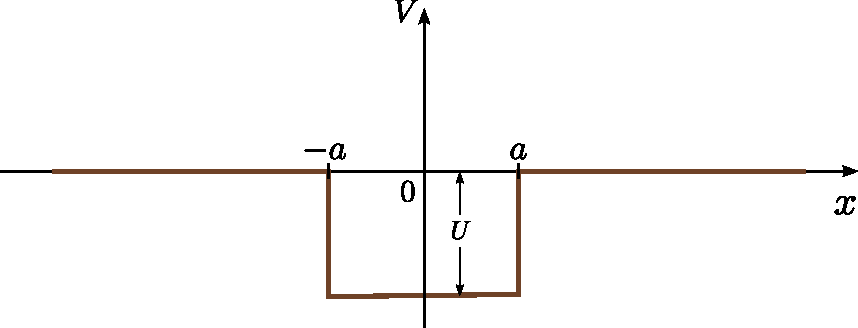
\includegraphics[width=0.57\textwidth]{squarewell}
\end{figure}

We can solve the time-independent Schr\"odinger wave equation for this
Hamiltonian using a simple technique called the \textbf{transfer
  matrix method}.  Some key aspects of the calculation are described
below; the rest of the details are given in \textbf{Appendix B}.

Outside the potential well, the Schr\"odinger wave equation reduces to
\begin{equation}
  -\frac{\hbar^2}{2m}\,\frac{d^2\psi}{dx^2} = E \psi(x)
  \qquad (\text{for}\;\;|x| > a).  
  \label{eq:psioutside}
\end{equation}
For $E < 0$, we can find discrete solutions of the form
\begin{equation}
  \psi(x) = c_\pm\, e^{\mp\kappa x},\;\;\;\mathrm{where}\;\;
  c_\pm \in \mathbb{C}, \;\;
  \kappa = \sqrt{-\frac{2mE}{\hbar^2}} \in \mathbb{R}^+.
\end{equation}
By choosing $e^{-\kappa x}$ for $x > a$, and $e^{+\kappa x}$ for $x <
-a$, the wavefunction vanishes exponentially away from the potential
well, so it is normalizable to unity.  These solutions are called
bound states.  There is also a lower energy bound, $E \ge -U$,
stemming from the variational principle.  Hence, the bound states form
a discrete set of eigenenergies within the range
\begin{equation}
  -U \le E < 0.
\end{equation}

For $E > 0$, we cannot construct exponentially localized solutions.
We instead consider
\begin{equation}
  \psi(x) = \begin{cases} \alpha_-\, e^{ik x} + \beta_-\, e^{-ik x}, & \;\;\;x < -a\\ (\mathrm{something}) , & -a < x < a\\ \alpha_+\, e^{ik x} + \beta_+\, e^{-ik x} , & \;\;\,x > a,\end{cases}
  \quad\mathrm{where}\;\;\;
  k = \sqrt{\frac{2mE}{\hbar^2}} \in \mathbb{R}^+.
  \label{psiwaves}
\end{equation}
Such a solution is called a free state.  It cannot be normalized to
unity since $\int_{-\infty}^\infty |\psi(x)|^2 dx$ diverges.  However,
it is ``almost normalizable'' in the sense that $|\psi|^2$ does not
blow up as $|x| \rightarrow \pm\infty$.  We can thus treat it as a
valid quantum wavefunction, on the same footing as plane waves (the
wavefunctions for momentum eigenstates).

For each $E$, we can find coefficients $\alpha_\pm$ and $\beta_\pm$
for Eq.~\eqref{psiwaves} so as to satisfy the Schr\"odinger wave
equation.  It turns out that these four coefficients are not
independent; for example, if we fix $\alpha_\pm$, that uniquely
determines $\beta_\pm$ (see Appendix B).  As this can be done for all
$E \ge 0$, Eq.~\eqref{psiwaves} represents a continuous family of free
state solutions.

The following figure shows numerically obtained results for a square
well with $U = 30$ and $a=1$ (in units where $\hbar = m =1$).  The
energy spectrum is shown on the left side.  There are five discrete
bound states; their plots of $|\psi|^2$ versus $x$ are shown on the
right side.  These results were computed using the transfer matrix
method described in Appendix B.

\begin{figure}[h]
  \centering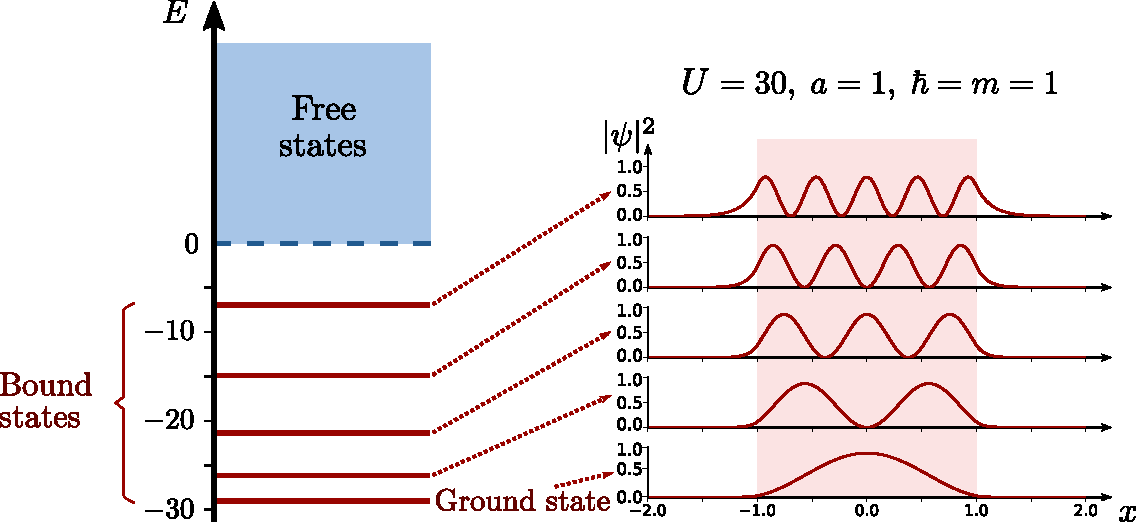
\includegraphics[width=0.72\textwidth]{boundvsextended}
\end{figure}

\clearpage
The number of bound states is not fixed.  In the figure below, we vary
the potential minimum $-U$ (with fixed $a = 1$), and plot the bound
state energies:

\vskip 0.15in
\begin{figure}[h]
  \centering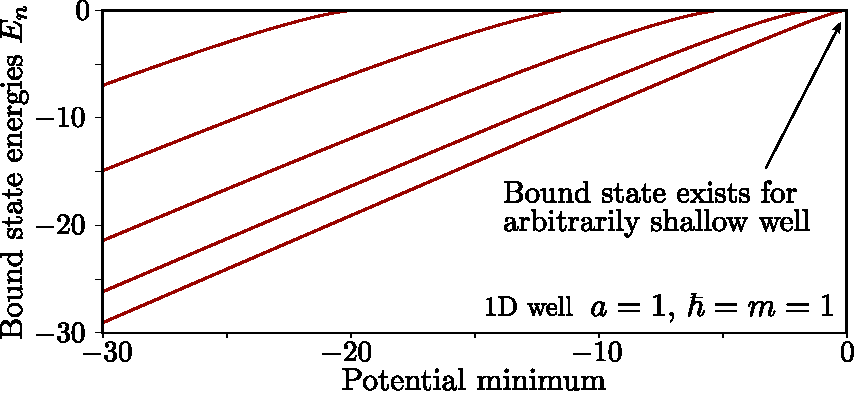
\includegraphics[width=0.68\textwidth]{boundstate1d}
\end{figure}

\noindent
For $U = 30$, there are five bound states.  As the well gets
shallower, these disappear one by one, with only one surviving as $U
\rightarrow 0$.  (There is a theorem stating that any 1D attractive
potential, no matter how weak, supports at least one bound state; see
\hyperref[ex:boundstate]{Exercise 1}.)

Many features of this simple model are generalizable to more
complicated cases, including higher spatial dimensions.  One notable
difference is that in 3D, it is possible for an attractive potential
to be too weak to support a bound state (i.e., its binding energy
cannot overcome the zero-point energy of a prospective ground state).
The figure below shows an example based on a uniform 3D spherically
symmetric well (the $l$ labels are angular momentum quantum numbers).
To learn more about this phenomenon, refer to
\hyperref[ex:boundstate3d]{Exercise 2}.

\vskip 0.15in
\begin{figure}[h]
  \centering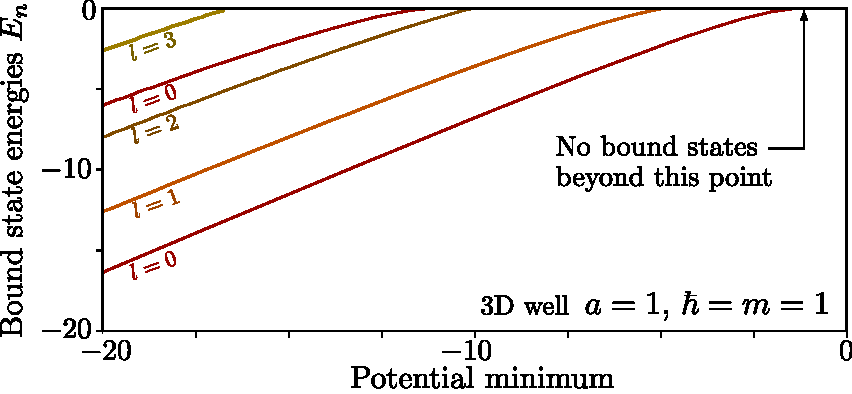
\includegraphics[width=0.68\textwidth]{boundstate3d}
\end{figure}

\section{Quasi-bound states and resonances}
\label{sec:resonances}

For the 1D finite square well, there is a clear distinction between
bound and free states.  However, certain states, called
``\textbf{quasi-bound states}'', can straddle the two cases.  As we
shall see, they play a particularly important important role in
scattering experiments.

The figure below shows an example of a potential function that hosts
quasi-bound states.  In the exterior region $|x| > b$, the potential
vanishes.  Between $x = -b$ and $x = b$, there is a barrier of height
$V_b$, in the middle of which is a well of depth $U < V_b$ and width
$2a$.  Since $V \ge 0$ everywhere, there are no bound states: all
eigenstates must be free states.

\begin{figure}[h]
  \centering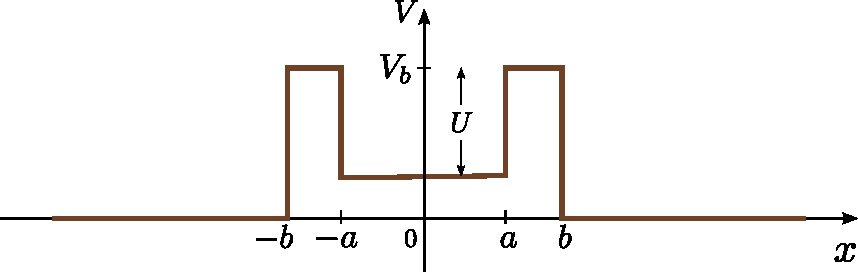
\includegraphics[width=0.62\textwidth]{resonancewell}
\end{figure}

There is something intriguing about the central well.  Consider an
alternative potential
\begin{equation}
  V_{\mathrm{alt}}(x) = \begin{cases}V_b - U, & |x| < a, \\ V_b, & \mathrm{otherwise},\end{cases}
\end{equation}
which is a finite square well.  This should have at least one bound
state, whose energy lies in the range $V_b-U < E < V_b$, and whose
wavefunction $\psi(x)$ decays exponentially away from the well.  Since
$V_{\mathrm{alt}}$ differs from the original potential $V$ only in the
region $|x| > b$, where $\psi(x)$ is small, this should also serve as
an \textit{approximate} solution for $V$!

In the context of the original scattering potential $V$, such a
solution is called a \textbf{quasi-bound state}.  It acts like a bound
state, but is not actually a bound state for $V$ (since it is not an
exact eigenstate).  In fact, as noted above, $V$ lacks true bound
states.

We can also analyze the situation using the scattering framework from
Chapter 1.  Consider an incident particle of energy $E > 0$ whose
wavefunction is
\begin{equation}
  \psi_i(x) = \Psi_i \, e^{ik_i x}.
\end{equation}
This produces a scattered wavefunction, which takes the following form
in the exterior region:
\begin{equation}
  \psi_s(x) = \Psi_i \times \begin{cases}f_- \,e^{-ik_ix}, & x \le -b \\ f_+ \,e^{ik_ix}, & x \ge b.\end{cases}
\end{equation}
We can obtain $f_\pm$ via the transfer matrix method (see Appendix B).
The figure below shows numerical results obtained for $U = 20,\,V_b =
30,\,a=1$, and $b \in \{ 1.2, 1.4\}$, with $\hbar = m = 1$.

\begin{figure}[h]
  \centering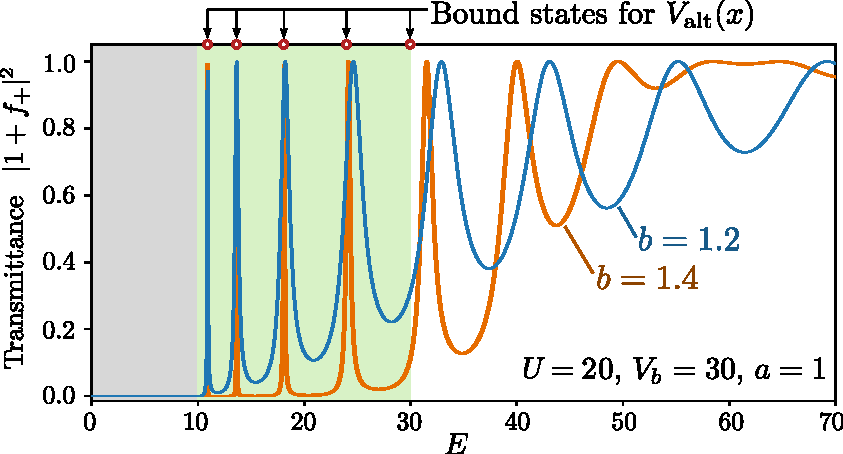
\includegraphics[width=0.62\textwidth]{resonances}
\end{figure}

The vertical axis shows the \textbf{transmittance} $|1+f_+|^2$, which
is the probability for the particle to pass through the scatterer.
The horizontal axis is the particle energy $E$.  Unsurprisingly, for
$E < V_b-U$ the transmittance approaches zero, and for $E \gtrsim V_b$
it approaches unity.  For $V_b-U < E \lesssim V_b$, the transmittance
forms a series of narrow peaks; for larger $b$ (i.e., when the central
well is more isolated from the exterior space), the peaks are
narrower.  At the top of the figure, we have also plotted the bound
state energies for the square well potential $V_{\mathrm{alt}}(x)$.
These energies closely match the locations of the transmittance peaks!

Looking at the wavefunction reveals other interesting features.
Below, we plot $|\psi(x)|^2$ versus $x$ at the energies of the first
three transmittance peaks, along with the corresponding quasi-bound
state wavefunctions.  At each peak, observe that: (i) $|\psi(x)|^2$ is
very large in the potential region, and (ii) its shape is very similar
to the corresponding quasi-bound state.

\begin{figure}[h]
  \centering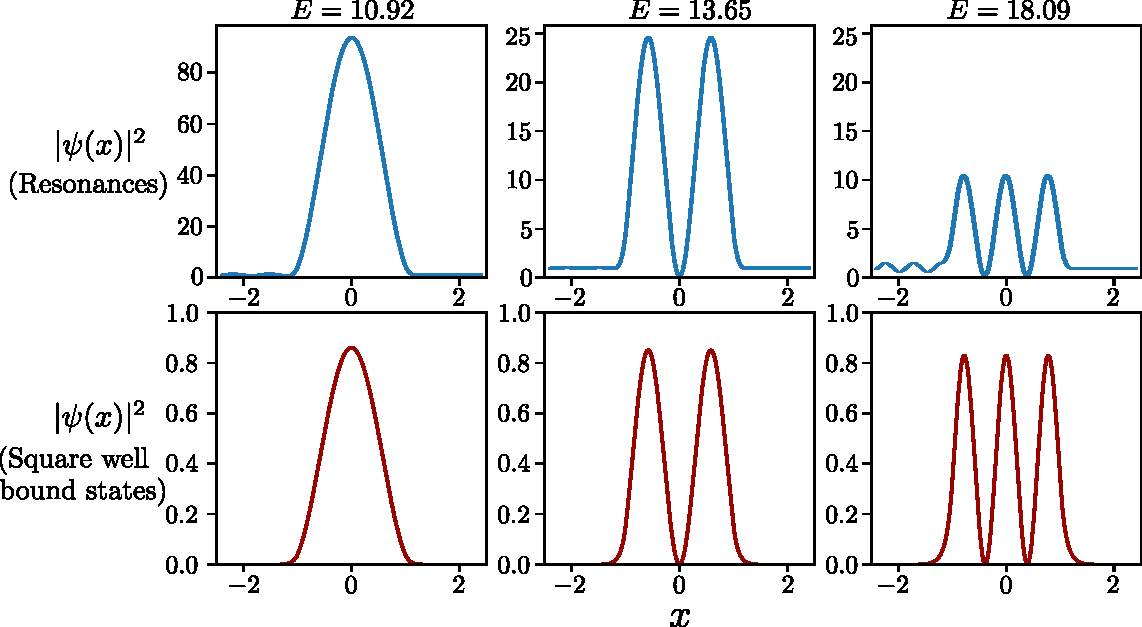
\includegraphics[width=0.83\textwidth]{resonancewavefunctions}
\end{figure}

\noindent
We interpret the situation as follows: at certain energies, an
incident particle ends up spending a long time trapped inside the
scatterer, taking on many of the characteristics of a bound state.
But unlike a true bound state, it is not trapped forever.  Eventually,
it leaks out of the scatterer and escapes to infinity.

The enhancement of $|\psi|^2$ by the presence of a quasi-bound state
is called \textbf{resonance}, and it is closely analogous to the
phenomenon of the same name in classical mechanics.  When a damped
harmonic oscillator is subjected to a periodic driving force, it
undergoes steady-state oscillation at the driving frequency.  If this
matches the frequency of one of the oscillator's ``normal modes'', the
oscillation amplitude grows large, as Galileo noted in the epigraph of
this chapter.

In the quantum scattering experiment, the incident wavefunction plays
the role of the driving force, $E$ acts as the driving frequency, and
quasi-bound states act like the normal modes.  Oftentimes, scattering
experiments are conducted for the express purpose of locating and
studying resonances.  When a resonance is found, it can be used to
deduce various important information about the scatterer, as we shall
see in the next few sections.

\section{Green's function analysis of scattering resonances}
\label{sec:green_resonances}

The Green's function formalism from Chapter 1, Sec.~1.5, provides a
powerful and general way to understand quasi-bound states and
resonances.  Notably, this framework applies not only to 1D models,
but works for higher dimensions as well.

Let $\hat{H} = \hat{T} + \hat{V}$ be the Hamiltonian of a system
supporting resonances, where $\hat{T}$ is the kinetic energy operator
and $\hat{V}$ is the potential operator.  We decompose the potential
into
\begin{equation}
  \hat{V} = \hat{V}_0 + \hat{V}_1,
  \label{Vdecomp}
\end{equation}
where $\hat{V}_0$ is a ``confining potential'' that supports a bound
state, and $\hat{V}_1$ is a ``deconfining potential'' that turns the
bound state into a quasi-bound state.  For example, the potential
functions for the 1D model of the previous section are shown below:

\begin{figure}[h]
  \centering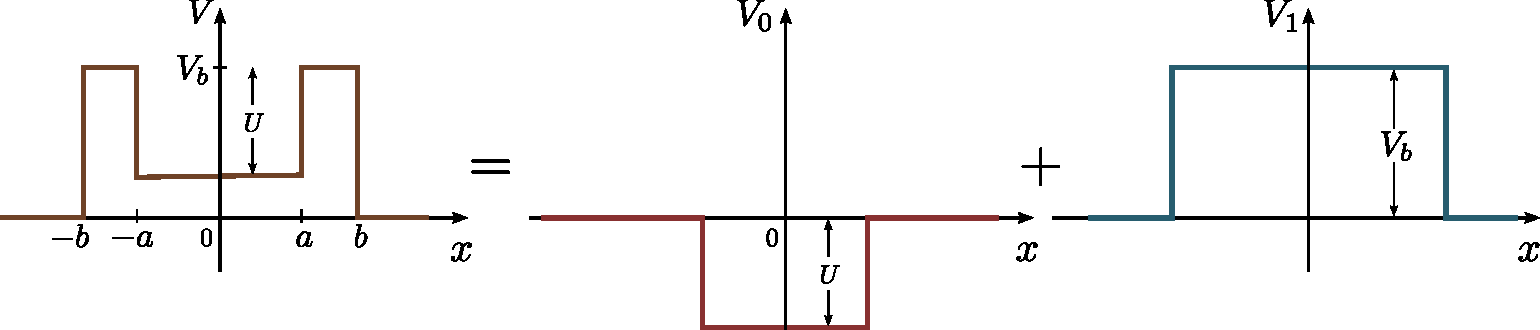
\includegraphics[width=0.95\textwidth]{resonancewell_decomp}
\end{figure}

\noindent
(Note that this 1D case is just an illustration; Eq.~\eqref{Vdecomp}
applies to higher dimensions too.)

When the potential is just $\hat{V}_0$, let there be a bound state
$|\varphi\rangle$ with energy $E_0$.  Furthermore, let us assume that
the potential supports a continuum of free states $\{|\psi_k\rangle\}$
with energies $\{E_k\}$, where $k$ is some continuous index for
labeling the free states (we will discuss what this index might
represent later).  The states satisfy the Schr\"odinger equation
\begin{align}
  \big(\hat{T} + \hat{V}_0\big) |\varphi\rangle \; &= E_0 |\varphi\rangle \\ \big(\hat{T} + \hat{V}_0\big) |\psi_k\rangle &= E_k |\psi_k\rangle,
\end{align}
along with the orthogonality and completeness relations
\begin{equation}
  \langle\varphi|\psi_k\rangle = 0, \;\;\quad |\varphi\rangle\langle\varphi|
  + \sum_k \, |\psi_k\rangle\langle\psi_k| = \hat{I}.
\end{equation}
Here, $\sum_k$ represents a sum over all free states.  Since the free
states form a continuum, this ought to be expressed as an integral,
similar to how we treat momentum eigenstates (see Chapter 1).  But,
for the moment, we write it as a sum for ease of presentation.

Let us treat $\hat{V}$ as a scattering potential, and compute the
Green's function.  According to Dyson's equations, the Green's
function for the full system is
\begin{equation}
  \hat{G} = \hat{G}_0 + \hat{G} \hat{V}_1 \hat{G}_0,
  \label{Gdyson}
\end{equation}
where
\begin{equation}
  \hat{G}_0(E) = \lim_{\varepsilon\rightarrow0^+}
  \Big(E - \hat{T} - \hat{V}_0 + i\varepsilon\Big)^{-1}
\end{equation}
is the causal Green's function.  Note that Eq.~\eqref{Gdyson} is
exact, not an approximation.  If we can obtain $\hat{G}(E)$, we can
determine the scattering amplitudes.

Let us find the matrix elements of $\hat{G}(E)$ by using
$|\varphi\rangle$ and $\{|\psi_k\rangle\}$ as a convenient basis.
Note, however, that this is \textit{not} the energy eigenbasis of
$\hat{H}$.

As usual when dealing with Dyson's equations, we must beware of the
fact that $\hat{G}$ appears on both the left- and right-hand sides.
We judiciously insert a resolution of the identity as follows:
\begin{align}
  \begin{aligned}
    \hat{G} \;=\; \hat{G}_0 + \hat{G} \hat{I} \hat{V}_1 \hat{G}_0
    \;=\; \hat{G}_0 + \hat{G} \left(|\varphi\rangle\langle\varphi|
    + \sum_k\, |\psi_k\rangle\langle\psi_k|\right) \hat{V}_1 \hat{G}_0.
  \end{aligned}
\end{align}
We then compute the matrix element
$\langle\varphi|\cdots|\varphi\rangle$ for both sides:
\begin{align}
    \langle\varphi|\hat{G}|\varphi\rangle = \langle\varphi|\hat{G}_0|\varphi\rangle &+ \langle\varphi|\hat{G}|\varphi\rangle \, \langle\varphi|\hat{V}_1 \hat{G}_0|\varphi\rangle + \sum_k\, \langle\varphi|\hat{G}|\psi_k\rangle \, \langle\psi_k| \hat{V}_1 \hat{G}_0|\varphi\rangle \nonumber\\
    \langle\varphi|\hat{G}|\varphi\rangle \left(1 - \langle\varphi|\hat{V}_1 \hat{G}_0|\varphi\rangle\right) &= \langle\varphi|\hat{G}_0|\varphi\rangle + \sum_k \, \langle\varphi|\hat{G}|\psi_k\rangle \, \langle\psi_k| \hat{V}_1 \hat{G}_0|\varphi\rangle \nonumber\\
    \lim_{\varepsilon\rightarrow0^+}
    \langle\varphi|\hat{G}|\varphi\rangle \left(1 - \frac{\langle\varphi|\hat{V}_1|\varphi\rangle}{E - E_0 + i\varepsilon}\right) &= \lim_{\varepsilon\rightarrow0^+} \frac{1}{E  - E_0 + i\varepsilon} \left(1+ \sum_k \, \langle\varphi|\hat{G}|\psi_k\rangle \, \langle\psi_k| \hat{V}_1|\varphi\rangle \right) \nonumber\\
    \lim_{\varepsilon\rightarrow0^+} \langle\varphi|\hat{G}|\varphi\rangle \Big(E - E_0 -\, \langle\varphi|\hat{V}_1|\varphi\rangle \, & + i\varepsilon\Big) - \sum_k\, \langle\varphi|\hat{G}|\psi_k\rangle \, \langle\psi_k| \hat{V}_1|\varphi\rangle = 1. \label{psiGphi}
\end{align}
Similarly, computing the matrix element
$\langle\varphi|\cdots|\psi_k\rangle$ gives
\begin{align*}
  \begin{aligned}
\langle\varphi|\hat{G}|\psi_k\rangle &= \langle\varphi|\hat{G}_0|\psi_k\rangle + \langle\varphi|\hat{G}|\varphi\rangle \, \langle\varphi|\hat{V}_1 \hat{G}_0|\psi_k\rangle + \sum_{k'}\, \langle\varphi|\hat{G}|\psi_{k'}\rangle \, \langle\psi_{k'}| \hat{V}_1 \hat{G}_0|\psi_k\rangle \\
&= \lim_{\varepsilon\rightarrow0^+} \left(E-E_k+i\varepsilon\right)^{-1} \left(\langle\varphi|\hat{G}|\varphi\rangle \, \langle\varphi|\hat{V}_1|\psi_k\rangle + \sum_{k'}\, \langle\varphi|\hat{G}|\psi_{k'}\rangle \, \langle\psi_{k'}| \hat{V}_1|\psi_k\rangle\right).\end{aligned}
\end{align*}

So far, the equations have been exact, but now we apply an
approximation: in the last line of the above equation, let the factor
of $\langle\varphi|G|\varphi\rangle$ be large, so that the first term
in the sum is dominant.  It will be shown below that
$\langle\varphi|G|\varphi\rangle$ being large is precisely the
resonance condition, so this approximation will be self-consistent.
Thus, we obtain
\begin{equation}
  \langle\varphi|\hat{G}|\psi_k\rangle \approx \lim_{\varepsilon\rightarrow0^+} \frac{\langle\varphi|\hat{G}|\varphi\rangle \, \langle\varphi|\hat{V}_1|\psi_k\rangle}{E-E_k+i\varepsilon}.
  \label{phiGpsi}
\end{equation}
Combining this with Eq.~\eqref{psiGphi} gives
\begin{equation*}
  \lim_{\varepsilon\rightarrow0^+} \left[\langle\varphi|\hat{G}|\varphi\rangle \left(E - E_0 -\, \langle\varphi|\hat{V}_1|\varphi\rangle \, + i\varepsilon\right) - \sum_k\, \frac{\langle\varphi|\hat{G}|\varphi\rangle\langle\varphi|\hat{V}_1|\psi_k\rangle}{E-E_k+i\varepsilon} \, \langle\psi_k| \hat{V}_1|\varphi\rangle\right] \approx 1.
\end{equation*}
We finally arrive at the result
\begin{framed}
  \begin{align}
    \langle\varphi|\,\hat{G}(E)\,|\varphi\rangle
    &\approx \frac{1}{\displaystyle E - E_0 - \langle\varphi|V_1|\varphi\rangle - \Sigma(E)}
    \label{phiGphi_result} \\
    \mathrm{where}\quad
    \Sigma(E) &\equiv \lim_{\varepsilon\rightarrow0^+}
    \sum_k \, \frac{\displaystyle| \langle\psi_k| \hat{V}_1|\varphi\rangle|^2}{\displaystyle E-E_k+i\varepsilon}.
    \label{sigma}
  \end{align}
\end{framed}

\section{The self energy}
\label{sec:self_energy}

The enigmatic $\Sigma(E)$ appearing in the denominator in
Eq.~\eqref{phiGphi_result} is called the \textbf{self energy}.  If we
put aside its dependence on $E$ and treat it as a constant,
Eq.~\eqref{phiGphi_result} looks like the Green's function of a system
with an energy eigenstate $|\varphi\rangle$ of energy
\begin{equation*}
  E_0 + \langle\varphi|\hat{V}_1|\varphi\rangle + \Sigma.
\end{equation*}
We can interpret this as the energy of the quasi-bound state.  The
first term is the energy of the original bound state, the second term
is a straightforward energy shift coming from the deconfining
potential $\hat{V}_1$, and the third term is the self energy.
According to Eq.~\eqref{sigma}, $\Sigma$ arises from the interplay
between $|\varphi\rangle$ and the free states $\{|\psi_k\rangle\}$.
The quasi-bound state disturbs the free states, which collectively
exert a back-action that shifts its energy.

There is an important complication: $\Sigma$ turns out to be complex,
not real!  From Eq.~\eqref{sigma},
\begin{align}
  \begin{aligned}\mathrm{Im}\big[\Sigma(E)\big] &= \lim_{\varepsilon\rightarrow0^+} \sum_k\, \Big| \langle\psi_k| \hat{V}_1|\varphi\rangle\Big|^2 \; \mathrm{Im}\left( \frac{1}{\displaystyle E-E_k+i\varepsilon}\right) \\ &= - \sum_k\, \Big| \langle\psi_k| \hat{V}_1|\varphi\rangle\Big|^2 \; \left[ \lim_{\varepsilon\rightarrow0^+} \; \frac{\varepsilon}{\displaystyle (E-E_k)^2 + \varepsilon^2}\right].\end{aligned}
\end{align}
The quantity in the square brackets is a Lorentzian function of
width $\varepsilon$.  The area under the curve is $\pi$, independent
of $\varepsilon$, so we can use the limiting expression
\begin{equation}
  \lim_{\varepsilon\rightarrow 0^+} \frac{\varepsilon}{x^2+\varepsilon^2} = \pi\delta(x).
\end{equation}
Therefore,
\begin{equation}
  \mathrm{Im}\big[\Sigma(E)\big]
  = - \pi \sum_k \; \big| \langle\psi_k| \hat{V}_1|\varphi\rangle\big|^2
  \; \delta(E-E_k) < 0.
  \label{fermigr1}
\end{equation}
What does it mean for an energy to be complex?  If a quantum state has
energy $E$, its time dependence goes as $\exp(-iE t/\hbar)$.  For $E =
\mathcal{E} + i \Gamma$, the time evolution factor is
\begin{equation*}
  e^{-i\mathcal{E} t/\hbar} \, e^{\Gamma t/\hbar}.
\end{equation*}
Since $\mathrm{Im}[\Sigma] < 0$, the quasi-bound state is decaying
exponentially with time.  This matches our description of it as a
localized state that is \textit{almost} an energy eigenstate, but not
exactly one---so, after some time, it escapes the scatterer and
disappears to infinity.

\section{Scattering resonances}
\label{sec:scattering_resonances}

In Chapter 1, Sec.~1.7, we derived the following relationship between
the Green's function and the scattering amplitude $f$:
\begin{equation}
  f(\mathbf{k}\rightarrow\mathbf{k}') \;\propto\; \langle \mathbf{k}'|\hat{V}|\mathbf{k}\rangle + \langle \mathbf{k}'|\hat{V}\hat{G}\hat{V}|\mathbf{k}\rangle.
\end{equation}
Here, $|\mathbf{k}\rangle$ and $|\mathbf{k}'\rangle$ are incident and
scattered plane wave states satisfying $|\mathbf{k}|=|\mathbf{k}'|$.
The first term describes the lowest-order scattering process (the
first Born approximation).  The second term contains second- and
higher-order scattering processes.

By inserting resolutions of the identity between each $\hat{V}$ and
$\hat{G}$ operator in the second term, we find that $f$ contains a
contribution of the form
\begin{equation}
  \Delta f(\mathbf{k}\rightarrow\mathbf{k}') \;\propto\; \langle \mathbf{k}'|\hat{V}|\varphi\rangle\langle\varphi|\hat{G}|\varphi\rangle\langle\varphi|\hat{V}|\mathbf{k}\rangle \;=\; \frac{\langle \mathbf{k}'|\hat{V}|\varphi\rangle \, \langle\varphi|\hat{V}|\mathbf{k}\rangle}{\displaystyle E - E_{\mathrm{res}} - i \mathrm{Im}[\,\Sigma\,]},
  \label{deltaf}
\end{equation}
where
\begin{equation}
  E_{\mathrm{res}} \;\equiv\; E_0 + \langle\varphi|\hat{V}_1|\varphi\rangle + \mathrm{Re}\big[\,\Sigma\,\big] \;\in\; \mathbb{R}.
  \label{Eres}
\end{equation}
At resonance, the denominator is small so $\Delta f$ is the dominant
part of $f$.  It is worth noting that $\Delta f$ contains
contributions from all terms in the Born series, not just low-order
terms.

The figure below shows the energy dependence of $\Delta f$, according
to Eq.~\eqref{deltaf}:

\begin{center}
  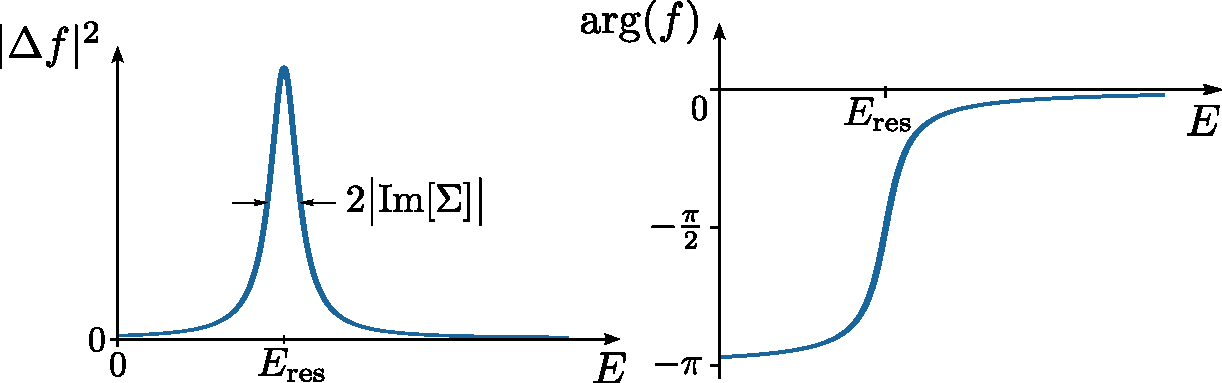
\includegraphics[width=0.69\textwidth]{resonance}  
\end{center}

\noindent
The graph of $|\Delta f|^2$ versus $E$ forms a Lorentzian curve
centered at $E_{\mathrm{res}}$.  The width of the peak can be
characterized by the full-width at half-maximum (FWHM), the spacing
between the two energies where $|\Delta f|^2$ has half its maximum
value, which can be calculated to be
\begin{equation}
  \delta E^{(\mathrm{FWHM})} = 2\, \big|\mathrm{Im}[\Sigma]\big|.
\end{equation}
(Note: we showed earlier that $\mathrm{Im}[\Sigma] < 0$.)  The smaller
the decay rate, the sharper the peak.

The phase $\mathrm{arg}[\Delta f]$ also contains useful information.
As $E$ crosses $E_{\mathrm{res}}$ from below, the phase increases by
$\pi$.  The shift also occurs over an energy width of $\sim
|\mathrm{Im}[\Sigma]|$.

These resonant features---peaks and/or phase shifts---are sought after
in many kinds of real-world scattering experiments.  Often, they are
overlaid on a ``background'' caused by non-resonant processes.  This
can be seen, for example, in the plot below from the CMS experiment at
the Large Hadron Collider (LHC), declaring the experimental
observation of the Higgs boson in 2012.

\begin{center}
  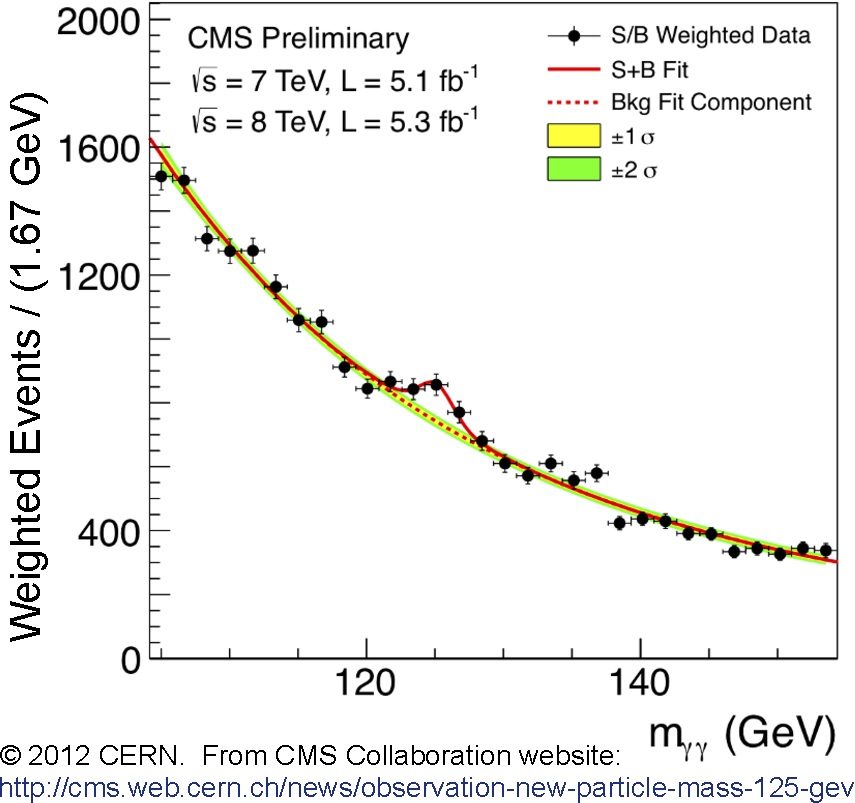
\includegraphics[width=0.4\textwidth]{higgs}
\end{center}

\section{Fermi's Golden Rule}
\label{sec:goldenrule}

In the previous sections, we have seen that the width of a resonance
is determined by the decay rate of a quasi-bound state, which is given
by the imaginary part of its self energy.  Now, we will derive a
simple and powerful formula for approximating it in many
circumstances, called \textbf{Fermi's Golden Rule}.

Suppose we initialize the particle, at time $t = 0$, to a quasi-bound
state $|\varphi\rangle$.  As $|\varphi\rangle$ is not an eigenstate of
the Hamiltonian, the particle does not remain in that state forever.
To quantify the ``decay'' of the quasi-bound state, we imagine
performing a measurement that has $|\varphi\rangle$ as one of its
eigenstates, at time $t > 0$.  The probability that the particle is
observed to still be in state $|\varphi\rangle$ is
\begin{equation}
  P(t) = \Big|\langle\varphi|\exp\left(-i\hat{H}t/\hbar\right)|\varphi\rangle\Big|^2.
\end{equation}
To help us calculate $P(t)$, let us define
\begin{equation}
  f(t) = \begin{cases} \langle\varphi|\exp\left(-i\hat{H}t/\hbar\right)|\varphi\rangle \,e^{-\varepsilon t}, & t \ge 0 \\ 0, & t < 0,\end{cases}
  \label{fregulated}
\end{equation}
where $\varepsilon \in \mathbb{R}^+$.  For $t \ge 0$ and $\varepsilon
\rightarrow 0^+$, we see that $|f(t)|^2 \rightarrow P(t)$.  The reason
we deal with $f(t)$ is that it is more well-behaved than the actual
amplitude $\langle\varphi|\exp(-i\hat{H}t/\hbar)|\varphi\rangle$.  The
function is designed so that (i) it vanishes at times prior to start
of the experiment, and (ii) it vanishes as $t\rightarrow\infty$ due to
the regulator $\varepsilon$.  The latter condition is based on our
expectation that the bound state should decay permanently into the
continuum of free states, and should never be repopulated by waves
``bouncing back'' from infinity.

To find $f(t)$, we first take its Fourier transform,
\begin{equation}
  F(\omega) \;=\; \int_{-\infty}^\infty dt \; e^{i\omega t}\, f(t) \;=\; \int_0^\infty dt \; e^{i(\omega + i\varepsilon) t} \; \langle\varphi|e^{-i\hat{H}t/\hbar}|\varphi\rangle.
\end{equation}
Now insert a resolution of the identity, $\hat{I} = \sum_n
|n\rangle\langle n|$, where $\{|n\rangle\}$ denotes the exact
eigenstates of $\hat{H}$ (for free states, the sum goes to an integral
in the usual way):
\begin{align}
  \begin{aligned}F(\omega) &= \int_0^\infty dt \; e^{i(\omega + i\varepsilon) t} \; \sum_n \langle\varphi|e^{-i\hat{H}t/\hbar}|n\rangle\langle n|\varphi\rangle \\ &= \sum_n \langle\varphi|n\rangle \left( \int_0^\infty dt \; \exp\left[i\left(\omega - \frac{E_n}{\hbar} + i\varepsilon\right) t\right] \right) \langle n|\varphi\rangle \\ &= \sum_n \langle\varphi|n\rangle \frac{i}{\omega - \frac{E_n}{\hbar} + i \varepsilon} \langle n|\varphi\rangle \\ &= i \hbar\; \langle \varphi | \left(\hbar\omega - \hat{H} + i\hbar\varepsilon \right)^{\!-1} | \varphi\rangle. \end{aligned}
\end{align}
In the third line, the regulator $\varepsilon$ removes the
contribution from the $t \rightarrow\infty$ limit.  Hence,
\begin{equation}
  \lim_{\varepsilon \rightarrow 0^+} F(\omega) = i \hbar \, \langle \varphi | \hat{G}(\hbar\omega) | \varphi\rangle,
\end{equation}
where $\hat{G}$ is our old friend the causal Green's function (see
Chapter 1, Sec.~1.6).  Its appearance can be traced to
Eq.~\eqref{fregulated}, which defines $f(t)$ to be nonzero only for $t
\ge 0$.

In Section~\ref{sec:scattering_resonances}, we saw that when the
system is at or close to resonance,
\begin{equation}
  \langle\varphi|\,\hat{G}(E)\,|\varphi\rangle \approx \frac{1}{\displaystyle E - E_{\mathrm{res}} - i \mathrm{Im}[\Sigma]},
\end{equation}
where $E_{\mathrm{res}}$ is the resonance energy, and $\Sigma$ is the
self energy of the quasi-bound state.  Using this, we can perform an
inverse Fourier transform to retrieve $f(t)$:
\begin{align}
  \begin{aligned} \lim_{\varepsilon\rightarrow 0^+} f(t) &= \lim_{\varepsilon\rightarrow 0^+} \int_{-\infty}^{\infty} \frac{d\omega}{2\pi} \; e^{-i\omega t} \, F(\omega) \\
    &\approx \frac{i}{2\pi} \int_{-\infty}^{\infty} d\omega\; \frac{e^{-i\omega t}}{\omega - (E_{\mathrm{res}}+i \mathrm{Im}[\Sigma])/\hbar} \\
    &\approx \exp\left(-\frac{iE_{\mathrm{res}}t}{\hbar}\right)\, \exp\left(-\frac{|\mathrm{Im}[\Sigma]|}{\hbar}\,t\right),
  \end{aligned}
\end{align}
where $\mathrm{Im}[\Sigma]$ is to be evaluated at $E =
E_{\mathrm{res}}$.  Thus,
\begin{equation}
  P(t) = e^{-\kappa t}, \;\;\;\mathrm{where}\;\;\kappa
  = \frac{2\big|\mathrm{Im}[\Sigma(E_{\mathrm{res}})]\big|}{\hbar}.
  \label{Ptresult}
\end{equation}
The quasi-bound state decays exponentially, with a decay rate
proportional to $|\mathrm{Im}[\Sigma]|$.

We previously derived a formula for $\mathrm{Im}[\Sigma]$,
Eq.~\eqref{fermigr1}, reproduced here for convenience:
\begin{equation}
  \mathrm{Im}\big[\Sigma(E)\big]
  = - \pi \sum_k \; \big| \langle\psi_k| \hat{V}_1|\varphi\rangle\big|^2
  \; \delta(E-E_k).
  \label{fermigr1a}
\end{equation}
In the sum over $k$, each term is a non-negative real number
consisting of two factors: (i) a $k$-dependent ``weight'' $|
\langle\psi_k| \hat{V}_1|\varphi\rangle|^2$, and (ii) a delta
function, which vanishes unless $E_k = E$.  Because only a subset of
the free states are relevant to the sum, it is convenient to define
\begin{equation*}
  \overline{\big| \langle\psi_{k(E)}| \hat{V}_1|\varphi\rangle\big|^2},
\end{equation*}
which is the average weight over the participating free states (i.e.,
those with $E = E_k$).  Then we can approximate Eq.~\eqref{fermigr1a}
by pulling the weights out of the sum:
\begin{equation}
  \mathrm{Im}\big[\Sigma(E)\big]
  \approx - \pi \;
  \overline{\big| \langle\psi_{k(E)}| \hat{V}_1|\varphi\rangle\big|^2}
  \; \sum_k \; \delta(E-E_k).
  \label{fermigr2}
\end{equation}
This allows us to write the decay rate in Eq.~\eqref{Ptresult} as
\begin{framed}
  \begin{equation}
    \kappa
    \,\approx\, \frac{2\pi}{\hbar} \;
    \overline{\big|W\big|^2} \; \rho(E_{\mathrm{res}}),
    \quad \mathrm{where} \quad \left\{
    \begin{aligned}
      W &= \langle\psi_{k}| \hat{V}_1|\varphi\rangle \\
      \rho(E) &= \sum_k \; \delta(E-E_k).
    \end{aligned}\right.
    \label{FGR}
  \end{equation}
\end{framed}
\vskip -0.1in
\noindent
This result is called \textbf{Fermi's golden rule}.  It states that
the decay rate of a quasi-bound state is determined by the product of
two real factors:

\begin{itemize}
\item
  $\overline{|W|^2}$, which is obtained by taking the absolute square
  of the \textbf{transition amplitude} $\langle\psi_{k}|
  \hat{V}_1|\varphi\rangle$, and averaging over available free states
  (i.e., the free states meeting the resonance condition $E_k =
  E_{\mathrm{res}}$).  This characterizes how strongly the quasi-bound
  state couples, on average, to the available free states.

\item
  $\rho(E_{\mathrm{res}})$, which is the number of free states per
  unit energy at energy $E_{\mathrm{res}}$.  This says that the decay
  rate is proportional to the number of available free states.
\end{itemize}
\vskip -0.1in
\noindent
Typically, these two factors are estimated by making further
approximations.

One very common approximation is to treat the free states as plane
waves.  In this case, we take the $k$ labels to be $d$-dimensional
wave-vectors.  As the wave-vectors are continuous, we convert the sum
over $k$ into an integral in the usual way, by defining the
discretization step $dk = 2\pi/L$ where $L \rightarrow \infty$ (see
Chapter 1, Sec.~1.2):
\begin{align}
  \rho(E) &= \sum_k \delta(E-E_k) \nonumber \\
  &= L^d \underbrace{\int \frac{d^d k}{(2\pi)^d} \; \delta(E - E_k).}_{\equiv \displaystyle \mathcal{D}(E)} \label{densityofstates}
\end{align}
The \textbf{density of states} $\mathcal{D}(E)$ counts the number of
free states of energy $E$, per unit energy and per unit volume.  Note
that it has different dimensions from $\rho(E)$.  We also need to
re-normalize the transition amplitude, via the usual
delta-normalization convention:
\begin{align}
  |\psi_k\rangle^{(\textrm{new})}
  &= \left(\frac{L}{2\pi}\right)^{d/2} |\psi_{k}\rangle^{(\textrm{old})} \\
  \Rightarrow \;\;\;
  \langle\psi_{k}| \hat{V}_1|\varphi\rangle^{(\textrm{old})}
  &= \left(\frac{2\pi}{L}\right)^{d/2} \langle\psi_{k}| \hat{V}_1|\varphi\rangle^{(\textrm{new})}.
  \label{psiknew}
\end{align}
Plugging Eq.~\eqref{densityofstates} and \eqref{psiknew} into
\eqref{FGR}, we can re-state Fermi's golden rule as
\begin{framed}
  \begin{equation}
    \kappa
    \,\approx\, \frac{2\pi}{\hbar} \;
    \overline{\big|\mathcal{W}\big|^2} \;
    \mathcal{D}(E_{\mathrm{res}}),
    \quad \mathrm{where} \quad \left\{
    \begin{aligned}
      \mathcal{W}
      &= (2\pi)^{d/2} \;
      \langle\psi_{k}| \hat{V}_1|\varphi\rangle \\
      \mathcal{D}(E) &= \int \frac{d^dk}{(2\pi)^d} \; \delta(E-E_k).
    \end{aligned}\right.
    \label{FGR2}
  \end{equation}
\end{framed}
\vskip -0.1in
\noindent
Here, $\overline{\big|\mathcal{W}\big|^2}$ is averaged over all plane
waves satisfying the resonance condition $E_k = E$.  Note that the $L$
factors in Eq.~\eqref{densityofstates} and \eqref{psiknew} do not
appear in the result \eqref{FGR2}, as they have cancelled each other
out.

\section{Fermi's golden rule in a 1D model}
\label{sec:fgr1d}

Let us apply Fermi's golden rule to the simple 1D model of
Section~\ref{sec:resonances}.  The potential is
\begin{equation}
  V(x) = V_0(x) + V_1(x), \;\;\;\mathrm{where}\;\;
  \left\{\;\;
  \begin{aligned}
    V_0(x) &= -U \, \Theta(a-|x|) \\
    V_1(x) &= \;\;V_b\; \Theta(b-|x|) \\
    0 &<U<V_b.
  \end{aligned}\right.
\end{equation}
The finite square well $V_0(x)$ supports one or more bound states; for
simplicity, we focus on the ground state, whose energy is denoted by
$E_0$ (where $-U < E_0 < 0$).  Its wavefunction is
\begin{equation}
  \varphi(x) = \begin{cases}\mathcal{A}\,\cos(qx), & |x| < a \\
    \mathcal{B} \, \exp\left(-\eta|x|\right), & |x| \ge a,\end{cases}
  \label{varphiansatz0}
\end{equation}
where $\mathcal{A}$ and $\mathcal{B}$ are constants to be determined,
and
\begin{equation}
  q = \sqrt{\frac{2m}{\hbar^2}(E_0+U)}, \;\; \eta = \sqrt{\frac{2m}{\hbar^2}|E_0|}.
\end{equation}
By matching $\varphi(x)$ and $d\varphi/dx$ across the $x=a$ interface,
we can derive $E_0$, $\mathcal{A}$, and $\mathcal{B}$.  The details
are left as an \hyperref[ex:1dfgr]{exercise}.

Having obtained $\varphi(x)$, we want the transition amplitude
$\langle\psi_k|\hat{V}_1|\varphi\rangle$, where $\psi_k(x)$ is a
representative free eigenstate of $V_0(x)$ that the quasi-bound state
decays to.  We can estimate this with a series of tricks.  First,
\begin{equation}
  \langle\psi_k|\hat{V}_1|\varphi\rangle \,=\, \int_{-\infty}^\infty dx \, \psi_k^*(x)\, V_1(x)\, \varphi(x) \,=\, V_b \int_{-b}^b dx \; \psi_k^*(x) \,\varphi(x).
\end{equation}
Next, because $\psi_k(x)$ and $\varphi(x)$ are orthogonal,
\begin{equation}
  \int_{-\infty}^\infty dx \; \psi_k^*(x) \,\varphi(x) = 0
  \;\;\;\Rightarrow \;\;\;  
  \int_{-b}^b dx \; \psi_k^*(x) \,\varphi(x) = - \int_{|x| > b} dx \; \psi_k^*(x) \,\varphi(x).
\end{equation}
The integration range consists of two pieces, $x > b$ and $x < -b$,
which can be interpreted as the decay of the quasi-bound state to the
left or right.  We assume these contribute equally to the escape
probability, so
\begin{equation}
  \big| \langle\psi_k|\hat{V}_1|\varphi\rangle \big|^2
  \;\approx\; 2 V_b^2 \;
  \left| \int_{b}^\infty dx \, \psi_k^*(x)\, \varphi(x)\right|^2.
  \label{overlapintegral}
\end{equation}
Outside the scatterer, the escaping free state is approximately an
outgoing plane wave,
\begin{equation}
  \psi_k(x) \,\approx\, \frac{e^{ikx}}{\sqrt{2\pi}},
  \label{psikx}
\end{equation}
where
\begin{equation}
  E_k = E_{\mathrm{res}} \approx E_0 + V_b \;\;\;\Rightarrow \;\;\; k \approx \sqrt{\frac{2m}{\hbar^2}(E_0+V_b)}.
\end{equation}
Plugging Eqs.~\eqref{varphiansatz0} and \eqref{psikx} into
Eq.~\eqref{overlapintegral}, and solving the integral, gives
\begin{equation}
  \big| \langle\psi_k|\hat{V}_1|\varphi\rangle \big|^2
  \;\approx \; \frac{1}{\pi}\, V_b^2 \, \mathcal{B}^2\,
  \frac{e^{-2\eta b}}{k^2 + \eta^2}.
  \label{overlap1d}
\end{equation}

The other quantity we need for Fermi's golden rule is the density of
free states.  This can be found by taking $E_k \approx \hbar^2k^2/2m$,
and performing a change of variables:
\begin{align}
  \mathcal{D}(E)
  &= \int_{-\infty}^\infty \frac{dk}{2\pi} \; \delta\left(E-\frac{\hbar^2k^2}{2m}\right) \\
  &= 2 \cdot \frac{1}{2\pi} \int_0^\infty dE' \, \frac{dk}{dE'} \, \delta(E-E') \label{dos1d_0} \\
  &= \sqrt{\frac{m}{2\pi^2\hbar^2 E}}.
  \label{dos1d}
\end{align}
In Eq.~\eqref{dos1d_0}, the factor of 2 accounts for the fact that for
each $E$, both positive and negative $k$ contribute to the density of
states.

We can now plug Eqs.~\eqref{overlap1d} and \eqref{dos1d} into Fermi's
golden rule, Eq.~\eqref{FGR2}.  The figure below shows results for $U
= 6$, $V_b = 30$, and $a = 1$, with computational units $\hbar = m =
1$.  The orange curve shows how $\kappa$, the decay rate from Fermi's
golden rule, varies with the barrier thickness $b-a$.  For comparison,
the blue dots show the values of $\kappa$ derived from the resonant
scattering peak (see Section~\ref{sec:scattering_resonances}), by
computing the transmittance using the transfer matrix method (see
\textbf{Appendix B}) and numerically extracting the peak width.

\begin{figure}[h]
  \centering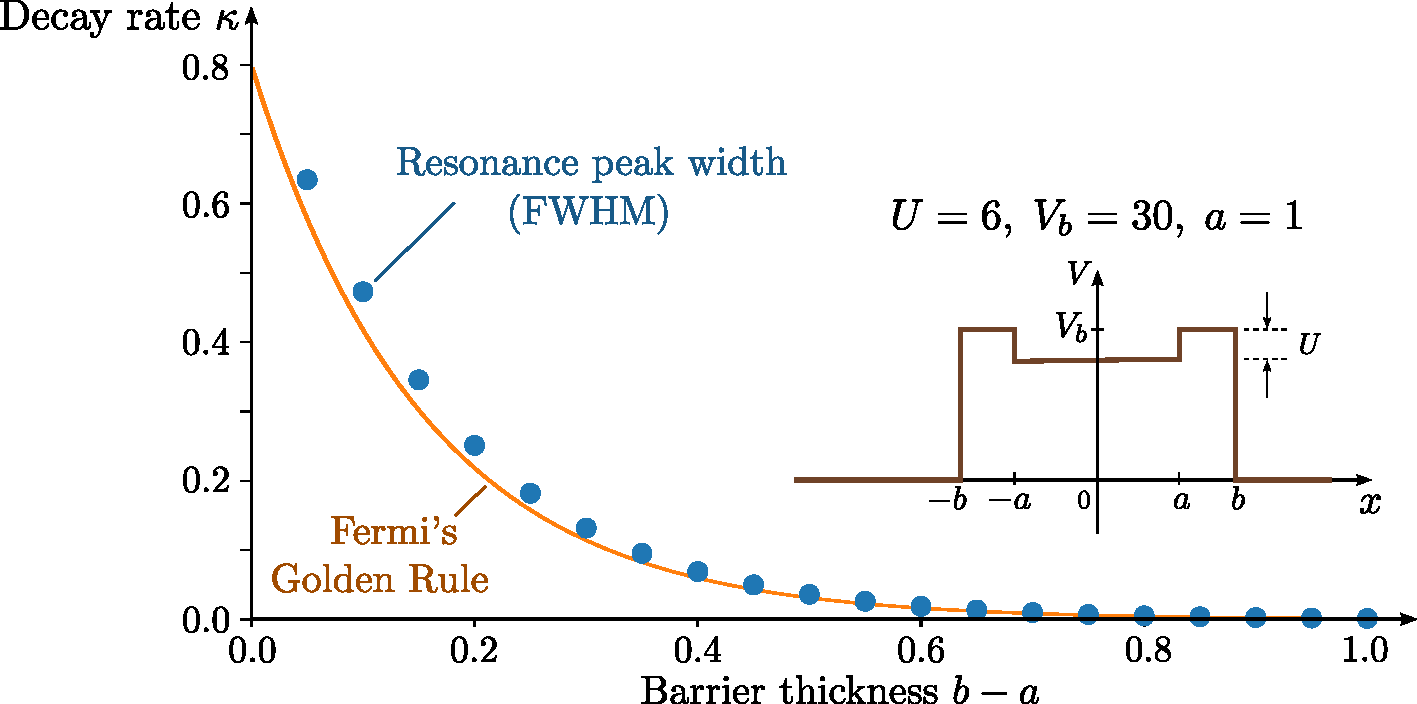
\includegraphics[width=0.8\textwidth]{goldenrule}
\end{figure}

\noindent
The agreement is pretty good, especially considering the numerous
approximations leading to the derivation of Fermi's golden rule!  The
behavior also matches our intuition: when the barrier thickness is
large, the quasi-bound state should indeed decay more slowly.

In this simple 1D example, Fermi's golden rule is not especially
useful since the scattering problem can be solved easily (see Appendix
B).  However, in higher dimensions, nonperturbative scattering
problems are typically much less tractable.  In such cases, Fermi's
golden rule provides a very convenient way to estimate the widths of
resonance peaks.

\section*{Exercises}

\begin{enumerate}
\item Use the variational theorem to prove that a 1D potential well
  has at least one bound state.  Assume that the potential $V(x)$
  satisfies (i) $V(x) < 0$ for all $x$, and (ii) $V(x)\rightarrow 0$
  for $x\rightarrow\pm\infty$.  The Hamiltonian is
  \begin{equation}
    \hat{H} = - \frac{\hbar^2}{2m} \frac{d^2}{dx^2} + V(x).
  \end{equation}
  Consider a (real) trial wavefunction
  \begin{equation}
    \psi(x;\gamma) = \left(\frac{2\gamma}{\pi}\right)^{1/4} \,e^{-\gamma x^2}.
  \end{equation}
  Note that this can be shown to be normalized to unity, using Gauss'
  integral
  \begin{equation}
    \int_{-\infty}^{\infty} dx\; e^{-2\gamma x^2} = \sqrt{\frac{\pi}{2\gamma}}.
  \end{equation}
  Now prove that
  \begin{align}
    \begin{aligned}
      \langle E \rangle &= \int_{-\infty}^\infty dx \; \psi(x) \, \hat{H} \,\psi(x) \\
      &= \frac{\hbar^2}{2m} \int_{-\infty}^\infty dx\, \left(\frac{d\psi}{dx}\right)^2
      \;+\; \int_{-\infty}^\infty dx\; V(x) \,\psi^2(x) \\
      &= A\sqrt{\gamma} \left[\sqrt{\gamma}
        \;+\, B \int_{-\infty}^\infty dx\; V(x) \;e^{-\gamma x^2}
        \right],
    \end{aligned}
  \end{align}
  where $A$ and $B$ are positive real constants to be determined.  By
  looking at the quantity in square brackets in the limit $\gamma
  \rightarrow 0$, argue that $\langle E \rangle < 0$ in this limit.
  Hence, explain why this implies the existence of a bound state.

  Finally, try generalizing this approach to the case of a 2D
  radially-symmetric potential well $V(x,y) = V(r)$, where $r =
  \sqrt{x^2+y^2}$.  Identify which part of the argument fails in 2D.
       [For a discussion of certain 2D potential wells that
         \textit{do} always support bounds states, similar to 1D
         potential wells, see Ref.~[\ref{cite:simon}].]
  \label{ex:boundstate}

\item In this problem, you will investigate the existence of bound
  states in a 3D potential well that is finite, uniform, and
  spherically-symmetric.  The potential function is
  \begin{equation}
    V(r,\theta,\phi) = -U\Theta(a-r),
  \end{equation}
  where $a$ is the radius of the spherical well, $U$ is the depth,
  and $(r,\theta,\phi)$ are spherical coordinates defined in the usual
  way.

  The solution involves a variant of the partial wave analysis
  discussed in Appendix A.  For $E < 0$, the Schr\"odinger equation
  reduces to
  \begin{equation}
    \begin{cases}\Big(\nabla^2 + q^2\Big) \psi(r,\theta,\phi) = 0 \;\;\mathrm{where}\;\; q = \sqrt{2m(E+U)/\hbar^2}, \;\;&\mathrm{for} \; r \le a \\ \Big(\nabla^2 - \gamma^2\Big) \psi(r,\theta,\phi) = 0 \;\;\mathrm{where}\;\; \gamma = \sqrt{-2mE/\hbar^2}, \;\;&\mathrm{for} \; r \ge a. \end{cases}
  \end{equation}
  For the first equation (called the Helmholtz equation), we seek
  solutions of the form
  \begin{equation}
    \psi(r,\theta,\phi) = f(r) \, Y_{\ell m}(\theta,\phi),
  \end{equation}
  where $Y_{\ell m}(\theta,\phi)$ are
  \href{https://en.wikipedia.org/wiki/Spherical_harmonics}{spherical
    harmonics}, and the integers $l$ and $m$ are angular momentum
  quantum numbers satisfying $l \ge 0$ and $-l \le m \le l$.
  Substituting into the Helmholtz equation yields
  \begin{equation}
    r^2\frac{d^2f}{dr^2} + 2r \frac{df}{dr}+\left[q^2r^2-l(l+1)\right] f(r) = 0,
  \end{equation}
  which is the \textbf{spherical Bessel equation}.  The solutions to
  this equation that are non-divergent at $r = 0$ are $f(r) =
  j_\ell(qr)$, where $j_\ell$ is called a \textbf{spherical Bessel function
    of the first kind}.  Most numerical packages provide functions to
  calculate these (e.g.,
  \href{https://docs.scipy.org/doc/scipy/reference/generated/scipy.special.spherical_jn.html}{\texttt{scipy.special.spherical\_jn}}
  in \href{https://scipy.org/}{Scientific Python}).

  Similarly, solutions for the second equation can be written as
  $\psi(r,\theta,\phi) = g(r) \, Y_{\ell m}(\theta,\phi),$ yielding an
  equation for $g(r)$ called the \textbf{modified spherical Bessel
    equation}.  The solutions which do not diverge as $r\rightarrow
  \infty$ are $g(r) = k_\ell(\gamma r)$, where $k_\ell$ is called a
  \textbf{modified spherical Bessel function of the second kind}.
  Again, this can be computed numerically (e.g., using
  \href{https://docs.scipy.org/doc/scipy/reference/generated/scipy.special.spherical_kn.html#scipy.special.spherical_kn}{\texttt{scipy.special.spherical\_kn}}
  in Scientific Python).

  Using the above facts, show that the condition for a bound state to
  exist is
  \begin{equation}
    \frac{qj_\ell'(qa)}{j_\ell(qa)} = \frac{\gamma k_\ell'(\gamma a)}{k_\ell(\gamma a)},
  \end{equation}
  where $j_\ell'$ and $k_\ell'$ denote the derivatives of the relevant
  special functions, and $q$ and $\gamma$ depend on $E$ and $U$ as
  described above.  Write a program to search for the bound state
  energies at any given $a$ and $U$, and hence determine the
  conditions under which the potential does not support bound
  states.
\label{ex:boundstate3d}

\item
  \label{ex:1dfgr}
  In this problem, we will find the quasi-bound and free states for
  the model discussed in Section~\ref{sec:fgr1d}, and use it to
  calculate the decay rate according to Fermi's golden rule.

  Let $\varphi(x)$ be the bound state of a square well of width $2a$
  and depth $U$, and let $E_0$ be the energy.  This state satisfies
  the 1D time-independent Schr\"odinger wave equation,
  \begin{equation}
    \left[- \frac{\hbar^2}{2m} \frac{d^2}{dx^2} + V(x)\right] \varphi(x)
    = E_0\, \varphi(x),
    \label{tise1d}
  \end{equation}
  where
  \begin{equation}
    V(x) = V_0(x) + V_1(x), \;\;\;\mathrm{where}\;\;
    \left\{\;\;
    \begin{aligned}
      V_0(x) &= -U \, \Theta(a-|x|) \\
      V_1(x) &= \;\;V_b\; \Theta(b-|x|) \\
      0 &<U<V_b.
    \end{aligned}\right.
    \label{vx}
  \end{equation}
  Take the ansatz
  \begin{equation}
    \varphi(x) = \begin{cases}\mathcal{A}\,\cos(qx), & |x| < a \\
      \mathcal{B} \, \exp\left(-\eta|x|\right), & |x| \ge a.\end{cases}
    \label{varphiansatz}
  \end{equation}

  \begin{enumerate}[(a)]
  \item Using Eqs.~\eqref{tise1d}--\eqref{varphiansatz}, and the fact
    that both $\varphi(x)$ and $d\varphi/dx$ are continuous at $x =
    \pm a$, prove that $E_0$ can be obtained by solving the
    transcendental equation
    \begin{align}
      q \tan(qa) = \eta, \;\;\;\mathrm{where}\;\;
      \left\{\;
      \begin{aligned}
        q &= \sqrt{\frac{2m}{\hbar^2}(E_0+U)} \\
        \eta &= \sqrt{\frac{2m}{\hbar^2}|E_0|}.
      \end{aligned}\right.
      \label{qtanqa}
    \end{align}
  
  \item By using the fact that $\varphi(x)$ is normalized to unity,
    prove that
  \begin{equation}
  \mathcal{B}^2 = \frac{\exp\big(2\eta a\big)}{a} \left[\frac{1+\sin(2qa)/2qa}{\cos^2(qa)}+\frac{1}{\eta a}\right]^{-1}.
  \label{Bresult}
  \end{equation}

\item Write a program to compute the decay rate based on Fermi's
  golden rule, by combining Eqs.~\eqref{FGR2}, \eqref{overlap1d},
  \eqref{dos1d}, \eqref{qtanqa}, and \eqref{Bresult}.  Hence,
  reproduce the plot shown in Section~\ref{sec:fgr1d}.

\item Write a program to extract the decay rate from the width of the
  transmission peak, using the transfer matrix method (see Appendix
  B).  Hence, investigate the accuracy of the Fermi's golden rule
  result for different values of $U$, $V_b$, and the other model
  parameters.

  \end{enumerate}

  





\end{enumerate}




\section*{Further Reading}

\begin{enumerate}[[1{]}]
\item Bransden \& Joachain, \S4.4, 9.2--9.3, 13.4
\item Sakurai, \S5.6, 7.7--7.8

\item R.~Courant and D.~Hilbert, \textit{Methods of Mathematical
  Physics} vol.~1, Interscience (1953).  [\href{https://archive.org/details/MethodsOfMathematicalPhysicsVolume1/page/n337}{link}]
  \label{cite:CourantHilbert}

\item B.~Simon, \textit{The bound state of weakly coupled
  Schr\"odinger operators in one and two dimensions}, Annals of
  Physics \textbf{97}, 279 (1976). [\href{https://doi.org/10.1016/0003-4916(76)90038-5}{link}]
\label{cite:simon}
\end{enumerate}

\end{document}


%% For decades after the discovery of quantum mechanics, the quantum
%% double-slit experiment was just a ``thought experiment'', meant to
%% illustrate the features of quantum mechanics that had been uncovered
%% by other, more complicated experiments.  Nowadays, the most convenient
%% way to do the experiment is with light, using single-photon sources
%% and single-photon detectors.  Quantum interference has also been
%% demonstrated experimentally using electrons, neutrons, and even
%% large-scale particles such as buckyballs.
